\documentclass[a4paper,10pt]{article}
\usepackage[utf8]{inputenc}
\usepackage{xspace}
\usepackage{graphicx,graphics} 
\usepackage{color}
\usepackage{amsmath}
\usepackage{amsfonts}
\usepackage{amssymb}
\usepackage{amsthm}
\usepackage{algorithm}
\usepackage{algorithmic}
\usepackage{longtable}
\usepackage{complexity}
\usepackage{tkz-graph}
\usepackage{float}
\usepackage{setspace}
\renewcommand{\algorithmicrequire}{\textbf{Input:}}
\renewcommand{\algorithmicensure}{\textbf{Output:}}
  
\graphicspath{{figures/}}
\newcommand\rmatching{${\cal R}$-matching\xspace}
\newcommand\mdelay{$\cal M$-delay\xspace}
\newcommand\matchedgraph{{\bf matched graph}}
\newtheorem{proposition}{Proposition}
\newtheorem{theorem}{Theorem}

\setlength{\parskip}{1ex} % Espace entre les paragraphes

\newtheorem{fact}{Fact}
\newtheorem{lemma}[theorem]{Lemma}
\newtheorem{definition}{Definition}
\newtheorem{corollary}{Corollary}



\newcommand{\todo}[1]{{\color{red} TODO: {#1}}}


%opening
\title{Contention Management for 5G}
\author{DB,CC,MG,OM,YS}


\begin{document}

\maketitle

\begin{abstract}
This article treats about Contention Management for 5G.
\end{abstract}

\section{Introduction}
  \begin{itemize}
    \item Context and problematic
    \item Related works
    \item Article contribution
  \end{itemize}

  

\section{Model}

  \subsection{Definitions}
  

  
	We consider a directed graph $G=(V,A)$ modelling a network. Each arc  $(u,v)$ in $A$ is labeled by an integer $dl(u,v) \geq 1$ that we call the delay and
	which represents the number of time slots taken by a signal to go from $u$ to $v$ using this arc. 
	%Note that for any arc $(u,v)$, $Dl(u,v)=Dl(v,u)$. Dominique voulait être plus général, on mettera cette propriété dans notre topologie
	
      A {\bf route} $r$ in $G$ is a sequence of consecutive arcs $a_0, \ldots , a_{k-1}$, with $a_i=(u_i,u_{i+1}) \in A$. 
      We will often refer to the first element of the route as a source and the last as a target.
      
      The {\bf latency} of a vertex $u_i$ in $r$, with $i \geq 1$, is defined by $$\lambda(u_i,r)= \sum\limits_{0 \leq j <i} dl(a_j)$$ We also define $\lambda(u_0,r)=0$.
      The latency of the route $r$ is defined by $\lambda (r)= \lambda (u_k,r)$.
      

      A {\bf routing function} $\cal R$ in $G$ associates to each pair of vertices $(u,v)$ a route from $u$ to $v$. Let $\cal C$ be an {\bf assignment} in $G$, i.e., a set of couples of different vertices of $G$. We denote by $\cal R_{\cal C}$ the set of routes ${\cal R}(u,v)$ for any $(u,v)$ in $\cal C$. We call $\cal R_{\cal C}$ a {\bf routage graph}, it contains all the informations needed in the forthcoming problems (assignment, routes and delays of the arcs). 
      

      \todo{Si on s'en sert, ajouter ici que le routage est cohérent.}

   \subsection{Slotted time Model}
      Consider now a positive integer $P$ called the {\bf period}. In our problem, we send in the network
      messages with period $P$. The time will thus be cut into slices of $P$ discrete slots. Assume we send a message at the source of the route $r$, at the time slot $m$ in the first period, then a message will be sent at time slot $m$ at each new period. We define the first time slot at which the message reaches a vertex $v$ in this route by $t(v,r) = m + \lambda(v,r) \mod P$. 

      A message usually cannot be transported in a single time slot. We denote by $\tau$ the number 
      of consecutive slots necessary to transmit a message. Let us call $[t(v,r)]_{P,\tau}$ the set of time slots used by $r$ at a vertex $v$ in a period $P$, that is $[t(v,r)]_{P,\tau} = \{t(v,r) + i \mod P \mid 0 \leq i < \tau \}$. Usually $P$ and $\tau$ will be clear from the context and we will denote $[t(v,r)]_{P,\tau}$ by $[t(v,r)]$.
      
      
      A {\bf $(P,\tau)$-periodic affectation} of a routage graph $\cal R_{\cal C}$ is a sequence  ${\cal M}=(m_0, \ldots ,m_{c-1})$ of $n$ integers that we call {\bf offsets}, with $n$ the number of routes in $\cal R_{\cal C}$. The number $m_i$ represents the index of the first slot used in a period  by the route $r_i \in \cal R_{\cal C}$ at its source.
      A $(P,\tau)$-periodic affectation must have no {\bf collision} between two routes in $\cal R_{\cal C}$, that is $\forall (r_i, r_j) \in {\cal R_{\cal C}}^2, i \neq j$, % with $\tau$ the size (in number of consecutive slots) of each message that must be periodically sent on each route of ${\cal R}_{\cal C}$, 
      we have $$[t(u,r_i)] \cap [t(u,r_j)] = \emptyset .$$
      

%       Notice that the notion of $P$-periodic affectation \textbf{is not monotone} with regard to $P$. 
      As an example of a $(2,1)$-periodic affectation, let consider a routage graph with routes $\{r_i\}_{i=1,\dots,n}$, such that all pairs of routes intersect at a different edge.
      We set $\tau = 1$ and the delays are chosen so that if $r_i$ and $r_j$ have $v$ as first common vertex then we have $\lambda(v,r_i) - \lambda(v,r_j)=1$.There is a $(2,1)$-periodic affectation by setting all $m_i$ to $0$.

%       A {\bf conflict graph} represents the collision between the routes of $ {\cal R}_{\cal C}$. The vertices of a conflict graph $G = (V,E)$ are the routes of $ {\cal R}_{\cal C}$, and there is an edge between two vertices if and only if there is a common arc between the two routes in $ {\cal R}_{\cal C}$.
%       
%       Given $u$ and $v$ two vertices of the conflict graph, corresponding to two routes colliding in $ {\cal R}_{\cal C}$. The weight of an edge, $w(u,v)$, is the absolute value of the difference between the distance of the two routes between their respective source node and the collision point.
%       
%       A labeling $F$ of such a graph is an affectation of an integer to each vertex, such that for each vertex $u$, $f(u) \neq f(v)+w(u,v)\mod P$, where $v$ are the neighbors of $u$ in the conflict graph and $P$ our period.
      \begin{figure}[h]
       \begin{center}
      
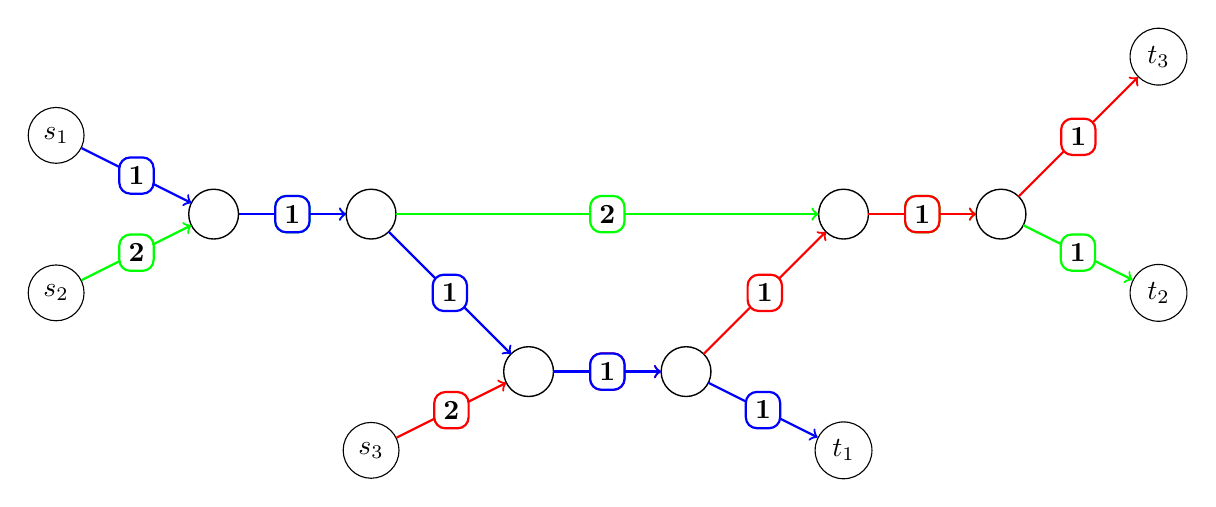
\begin{tikzpicture}


\tikzset{
  LabelStyle/.style = { rectangle, rounded corners, draw,
                       font = \bfseries },
  EdgeStyle/.append style = {->} }
  \SetGraphUnit{5}
  \node[draw,circle] (s3) at (4, 2) {$s_3$}; 
  \node[draw,circle] (s2) at (0, 4) {$s_2$}; 
  \node[draw,circle] (s1) at (0, 6) {$s_1$}; 

  \node[draw,circle] (t3) at (14, 7) {$t_3$}; 
  \node[draw,circle] (t2) at (14, 4) {$t_2$}; 
  \node[draw,circle] (t1) at (10, 2) {$t_1$}; 

  
  \SetVertexNoLabel
  \Vertex[x=2,y=5]{A}
  \Vertex[x=4,y=5]{B}
  \Vertex[x=10,y=5]{C}
  \Vertex[x=12,y=5]{D}
  \Vertex[x=6,y=3]{E}
  \Vertex[x=8,y=3]{F}
  \tikzset{
  EdgeStyle/.append style = {green} }
  \Edge[label = 2](s2)(A)
  \Edge[label = 1](A)(B)
  \Edge[label = 2](B)(C)
  \Edge[label = 1](C)(D)
  \Edge[label = 1](D)(t2)

  
   \tikzset{
  EdgeStyle/.append style = {red} }
  \Edge[label = 2](s3)(E)
  \Edge[label = 1](E)(F)
  \Edge[label = 1](F)(C)
  \Edge[label = 1](C)(D)
  \Edge[label = 1](D)(t3) 
     \tikzset{
  EdgeStyle/.append style = {blue} }
  \Edge[label = 1](s1)(A)
  \Edge[label = 1](A)(B)
  \Edge[label = 1](B)(E)
  \Edge[label = 1](E)(F)
  \Edge[label = 1](F)(t1)

\end{tikzpicture}
      \end{center}
       \caption{A routage graph with $(0,\dots,0)$ as a $(2,1)$-periodic affectation}
      \end{figure}




   \subsection{Problems}

    We want to ensure that there is an affectation which allows to send periodic messages from sources to target
    without collisions. The problem we need to solve is thus the following:
    

      \noindent {\bf  Periodic Routes Assignment (PRA)} 

      \noindent {\bf Input:} a routage graph $\cal R_{\cal C}$, an integer $\tau$ and an integer $P$.

      \noindent {\bf Question:} does there exist a $(P,\tau)$-periodic affectation of $\cal R_{\cal C}$ ?


      We will prove in Sec.~\ref{sec:complexity} that the problem PRA is $\NP$-complete, even in restricted settings.
      Even approximating the smallest value of $P$ for which there is a $(P,\tau)$-periodic affectation is hard.

      An unusual property of affectation is that given a routage graph, we may have a $(P,\tau)$-periodic affectation but no
      $(P',\tau)$-periodic affectation with $P' > P$: the existence of an affectation is not monotone with regards to $P$.

	\begin{lemma} 
	 For any odd $P$, there is a routage graph such that there is $(2,1)$-periodic affectation but no $(P,1)$-periodic affectation.
	\end{lemma}
\begin{proof}

      Consider the routage graph ${\cal R_{\cal C}}$ given in the previous subsection. 
      We change the delays so that for $v$, the first vertex which belongs to $r_i$ and $r_j$,
      we have $\lambda(v,r_i) - \lambda(v,r_j)= P$, where $P$ is an odd number smaller than $n$, the number of routes in ${\cal R_{\cal C}}$. In such a graph, there is no $(P,\tau)$-periodic affectation, because of $P < n$.\\
      If we consider a period of $2$, for all $i \neq j$, $\lambda(v,r_i) - \lambda(v,r_j) \mod 2 = 1$ . Therefore $(0,\dots,0)$ is a $(2,1)$-periodic affectation of ${\cal R_{\cal C}}$.

      
\end{proof}
      
% 
%       \begin{figure}[H]
%       \label{could-ran}
%       \begin{center}
%       % \begin{tabular}{cc}
%       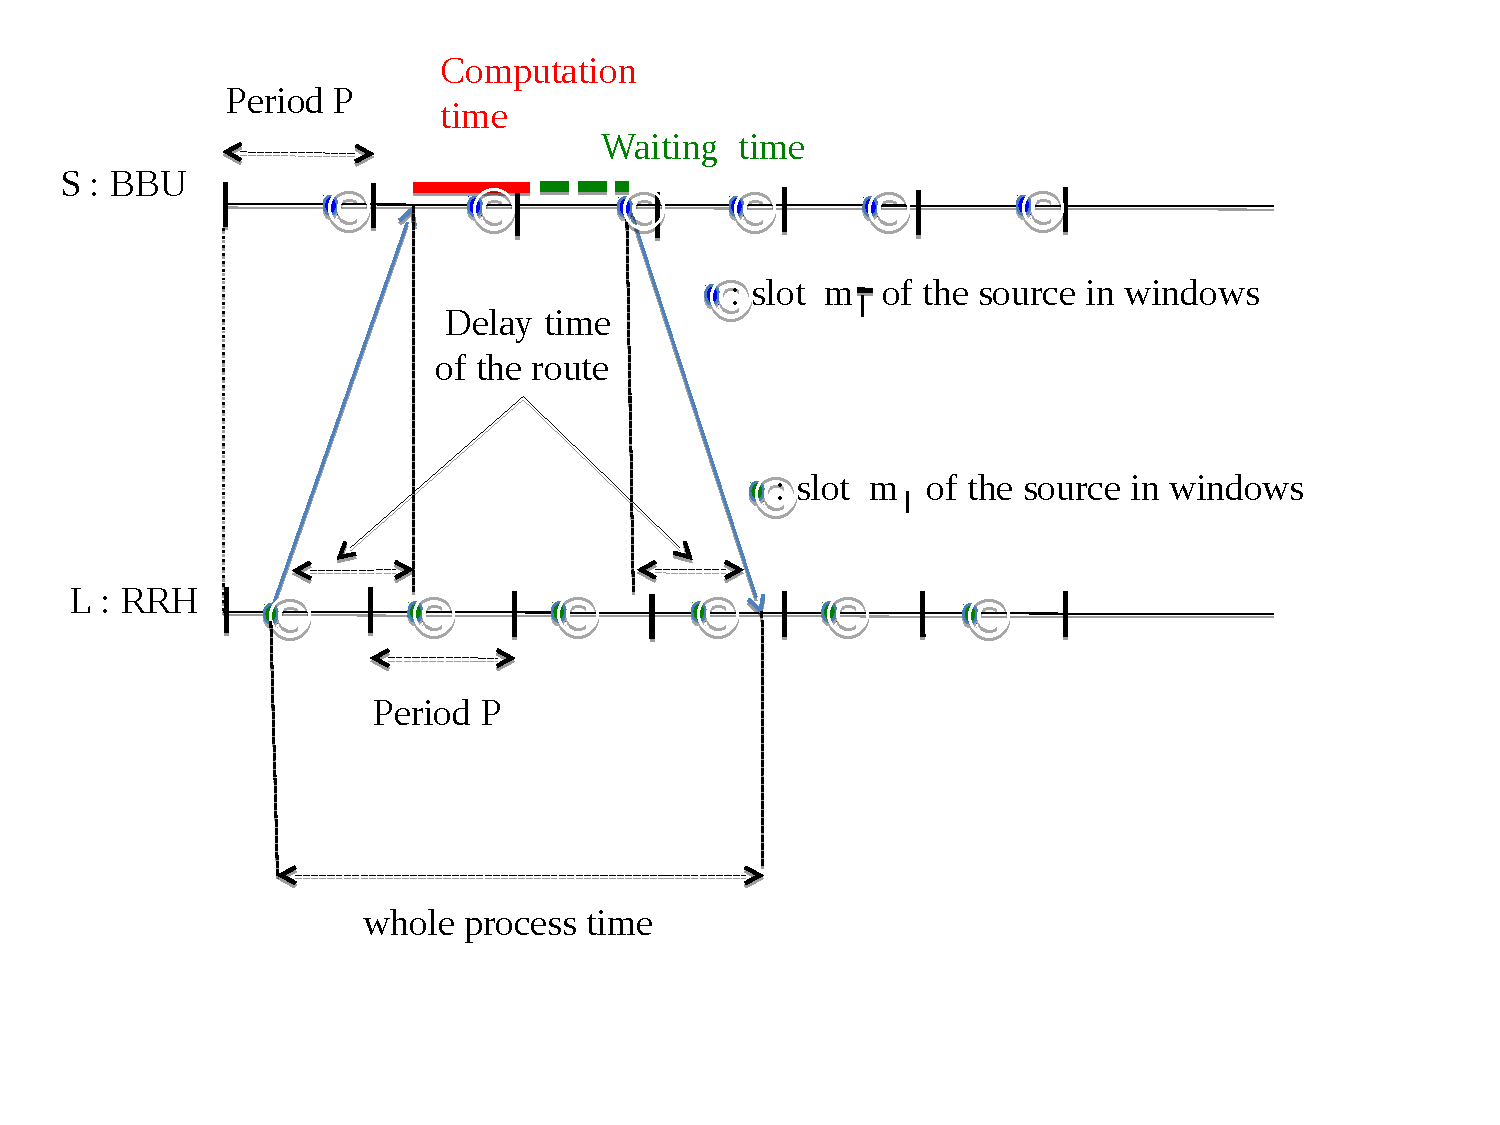
\includegraphics[scale=0.5]{Total-latence.pdf}
%       \caption{Complete process for a leaf in $L$.}
%       \end{center}
%       \end{figure}
%       %\end{tabular}\newline

      
      In the context of cloud-RAN applications, we consider here the digraph $G=(V,A)$ modeling the target network 
      and two disjoint subsets of vertices $S$ and $T$ of equal cardinality, where $S$ is the set of RRHs and $T$ is the set of BBUs. 
      A \textbf{symmetric} assignment ${\cal C}$, is an involutive function from $S$ to $T$, which maps each element $s\in S$ to ${\cal C}(s)$ and ${\cal C}(s)$ to $s$. It can also be seen as the set of pairs $(s,{\cal C}(s))$ and $({\cal C}(s),s)$.\\
      The Routing function ${\cal R}$ associates to each couple $(s,{\cal C}(s))$ a route called $r_s$ and to each couples $({\cal C}(s),s)$ a route called $r_{{\cal C}(s)}$.\\     
       We are given a period $P$, a routing function ${\cal R}$, and we consider a $(P,\tau)$-periodic affectation of ${\cal R}_{\cal C}$ which associates $m_s$ to the route $r_s$ which begins by $s$, and $m_{{\cal C}(s)}$ to the routes $r_{{\cal C}(s)}$ which begins by ${\cal C}(s)$.  This affectation represents the following process: first a message is sent at $s$, through the route $r_s$, at time $m_s$.
      
%       
%       We denote by $n$ the size of $S$ and $L$. We are given a period $P$, a routing function ${\cal R}$ and a bijection $\rho:L\rightarrow S$ which assigns a BBU to each RRH. Let ${\cal C}_{\rho} = \{(l,\rho(l))\}_{l \in L} \cup \{(s,\rho^{-1}(s))\}_{s \in S}$. Let consider a $P$-periodic affectation of ${\cal C}_{\rho}$ which associates $m_l$ to 
%       $(l,\rho(l))$ and $m_{\rho(l)}$ to $(\rho(l),l)$.  
      
      
      \begin{center}
      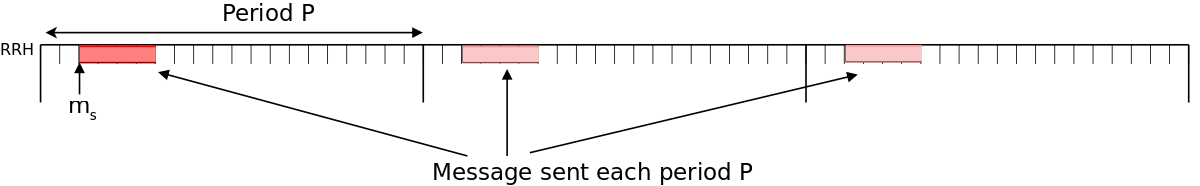
\includegraphics[scale=0.3]{rrh.png}
      \end{center}
      
      

      This message is received by ${\cal C}(s)$ at time $t({\cal C}(s),r_s)$. It is then sent back to $s$ in the same period at time $m_{{\cal C}(s)}$ if $m_{{\cal C}(s)} > t({\cal C}(s),r_s)$, otherwise at time $m_{{\cal C}(s)}$ in the next period. The time between the arrival of the message and the time it is sent back is called the \textbf{waiting time} and is defined by $w_s = m_{{\cal C}(s)} - t({\cal C}(s),r_s)$ if $m_{{\cal C}(s)} > t({\cal C}(s),r_s)$ and $w_s = m_{{\cal C}(s)} + P - t({\cal C}(s),r_s)$ otherwise.
      
       \begin{center}
      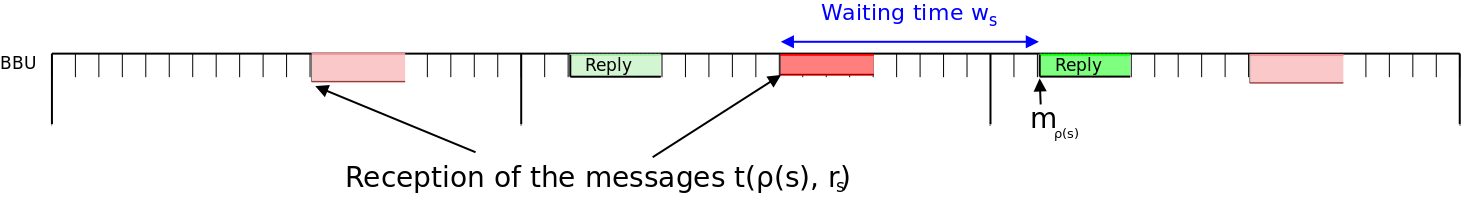
\includegraphics[scale=0.3]{BBU2.png}
      \end{center}
     

      When a BBU receives a message, it must compute the answer before sending it back to the RRH. This time can be encoded
      in the last arc leading to the BBU and thus we need not to consider it explicitly in our model.
    
      Thus, the whole process time for a message sent at vertex $s$ is equal to
      $$
      PT(s)=\lambda(r_s)+ w_s+\lambda(r_{{\cal C}(s)}).
      $$
      
    The {\bf maximum process time} of the $(P,\tau)$-periodic affectation ${\cal M} $ is defined by $MT({\cal M})=\max\limits_{s \in S} PT(s)$. The problem we want to solve is the following. 

      \noindent {\bf Periodic Assignment for Low Latency(PALL)} 

      \noindent {\bf Input:}  A routage graph ${\cal R}_{\cal C}$ with ${\cal C}$ a symmetric assignment, a period $P$, an integer $\tau$, an integer $T_{max}$.

      \noindent {\bf Question:} does there exist a $(P,\tau)$-periodic affectation ${\cal M}$ of ${\cal R}_{\cal C}$ such that $MT({\cal M}) \leq T_{max}$?

      \todo{Si on veut, on peut parler du temps moyen aussi ici, seulement si on fait quelque chose dessus dans la suite}
      %The related optimisation problem we will focus on  consists in minimizing  $MT({\cal M})$. Note that in the context of cloud-RAN networks, we consider $P=1ms$, $\theta=2.6ms$ and $T_{max}$ must be less or equal to $3ms$.
      %cette remarque doit être dans la partie expérimentale



  In this article, we works on given routages, but we could imagine a problem, in which, considering a given graph $G = (V,A)$ and a period P, the question is to find, if it exists, a routage graph ${\cal R}_{\cal C}$, in which there is $(P,\tau)$-periodic affectation.
\section{Solving PRA}
  \label{sec:complexity}
  \subsection{NP-Hardness}

 In this section we assume that the size of a message $\tau$ is equal to one. 
 We will prove the hardness of PRA and PALL for this parameter, which implies the hardness of the general problems. 
Consider an instance of the problem PRA, i.e., a routage graph $\cal{R_{\cal C}}$, a message size $\tau$ and a period $P$. \\
The {\bf conflict depth} of a route is the number of other routes which share an edge with it. 
The conflict depth of a routage graph  $\cal{R_{\cal C}}$ is the maximum of the conflict depth of the routes in $\cal{R_{\cal C}}$.\\
The {\bf load} of a routage graph is the maximal number of routes sharing the same arc.
It is clear that a $(P,\tau)$-periodic affectation must satisfy that $P$ is larger or equal to the load times $\tau$.


We give two alternate proofs that PRA is $\NP$-complete.
The first one works for conflict depth $2$ and is minimal in this regards since we later prove that for conflict depth one,
it is easy to solve PRA. The second one reduces the problem to graph coloring and implies inapproximability when one tries to minimize the parameter $P$. \\

 \begin{proposition}
Problem PRA is $\NP$-complete, when the routing is of conflict depth two.
\end{proposition}
 \begin{proof}
 The problem $PRA$ is in $\NP$ since given an offset for each route in an affectation, it is easy to check in linear time in the number of edges whether there are collisions.
 
  Let $H=(V,E)$ be a graph and let $d$ be its maximal degree. We consider the problem to determine whether $H$ is edge-colorable
  with $d$ or $d+1$ colors. The edge coloring problem is $\NP$-hard~\cite{holyer1981np} and we reduce it to PRA to prove its $\NP$-hardness. We define from $H$ an instance of PRA as follows. 
  For each $v$ in $V$, the graph $G$ has two vertices $v_1, v_2$, and for each $(u,v) \in E$,the graph g has two vertices $s_{u,v}, t_{u,v}$.
  
%   The set $A$ of arcs of $G$ is: 
%   $$ \{(v_1,v_2) \mid v\in V\} \cup \{(u_2,v_1)\mid u \neq v \in V^2\} \cup \{(s_{u,v},u_1),(v_2,t_{u,v}) \mid (u,v) \in E \}. $$
  For each edge $(u,v) \in E$, there is a route $s_{u,v},u_1,u_2,v_1,v_2,t_{u,v}$ in ${\cal R}$.  
  The set of arcs of G is the union between all the arcs of the previous routes.
  The affectation ${\cal C}$ is the set of pair of vertices $(s_{u,v}, t_{u,v})$.
  
  All these arcs are of weight $0$. 
  
    
  Observe that the existence of a $d$-coloring of $H$ is equivalent to the existence of a $(d,1)$-periodic affectation
  of ${\cal R}_{\cal C}$. Indeed, a $d$-coloring of $H$ can be seen as a labeling of its edges by the integers
  in $\{0,\dots,d-1\}$ and we have a bijection between $d$-colorings of $H$ and offsets of the routes of ${\cal R}_{\cal C}$.
  By construction, the constraint of having no collision between the routes is equivalent to the fact that no two adjacent edges have
  the same color. Therefore we have reduced edge coloring to PRA which concludes the proof. 
 \end{proof}
 \todo{Faire un dessin d'illustration ?}
 
 Remark that we have used zero weight in the proof. If we ask the weights to be strictly positive, which makes sense in our model since
they represent the latency of physical links, it is easy to adapt the proof. We just have to set them so that in any route the delay at $u_1$ is equal to $d$ and thus equal to $0$ modulo $d$. We now lift this hardness result to the problem PALL.

\begin{corollary}
Problem PALL is $\NP$-complete for routing of conflict depth two.
\end{corollary}
\begin{proof}
 We consider $({\cal R}_{\cal C},P,\tau)$ an instance of $PRA$. We assume that no vertex appears both in the first and second position in a pair of ${\cal C}$. Remark that this condition is satisfied in the previous proof, which makes the problem $PRA$ restricted to this kind of instances $\NP$-complete. 
 Let us define $T_{max} = 2 \times \max_{r \in {\cal R}} \lambda(r) + P$. We consider ${\cal C}'$ and ${\cal R}'_{\cal C'}$ symmetrized versions of ${\cal C}$ and  ${\cal R}_{\cal C}$ where for every route there is a symmetric route with new arcs and the same weights.
 The instance $({\cal R'}_{\cal C'},P,\tau,T_{max})$ is in PALL if and only if $({\cal R}_{\cal C},P,\tau)$
 is in $PRA$. Indeed the waiting time of each route is by definition less than $P$ and thus the maximal process time is always less than $T_{max}$. Moreover a $(P,\tau)$-affectation of ${\cal R}_{\cal C}$ can be extended into a $(P,\tau)$-affectation of ${\cal R'}_{\cal C'}$ in the following way. For each route $r_{u,v}$, the time at which the message arrives is $t(v,r_{u,v})$, then we choose as offset for $r_{v,u}$, $-t(v,r_{u,v}) \mod P$. The symmetry ensures that each new route $r_{v,u}$ in ${\cal R'}_{\cal C'}$ uses the same times slot as $r_{u,v}$ and thus avoid collisions.
\end{proof}

Let MIN-PRA be the problem, given a routage graph and an assignment, to find the minimal period $P$ such that there is a $P$-periodic affectation. 

\begin{theorem}
 The problem MIN-PRA cannot be approximated in polynomial time within a factor $n^{1-o(1)}$, with $n$ the number of routes, unless $\P = \NP$ even when the load is two.
\end{theorem}

\begin{proof}
 We reduce graph coloring to PRA. Let $H$ be a graph instance of the $k$-coloring problem. 
 We define ${\cal R}$ in the following way: for each vertex $v$ in $H$, there is a route $r_v$ in ${\cal R}$.
 Two routes $r_v$ and $r_u$ share an arc if and only if $(u,v)$ is an edge in $H$; this arc is the only one shared by these two routes.   
 All arcs are of delay $0$. 
 
 Observe that the existence of a $k$-coloring of $H$ is equivalent to the existence of a $(k,1)$-periodic affectation in $G$, 
 by converting an offset of a route into a color of a vertex and reciprocally. Therefore if we can approximate the minimum value of $P$ within some factor, we could approximate the minimal number of colors needed to color a graph within the same factor. The proof follows from the hardness of approximability of finding a minimal coloring~\cite{zuckerman2006linear}.
\end{proof}


In particular, this reduction shows that even with small maximal load, the 
minimal period can be large.

    \scalebox{0.5}{

    \begin{tikzpicture}

    \tikzset{
      LabelStyle/.style = { rectangle, rounded corners, draw,
			  font = \bfseries },
      EdgeStyle/.append style = {->} }
      \SetGraphUnit{5}
      \Vertex[x=4,y=2]{s3}
      \Vertex[x=0,y=4]{s2}
      \Vertex[x=0,y=6]{s1}
      
      \Vertex[x=12,y=3]{t3}
      \Vertex[x=14,y=4]{t2}
      \Vertex[x=10,y=2]{t1}
      \tikzstyle{VertexStyle}=[shape = circle, draw, minimum size = 20pt]
	\tikzset{
      VertexStyle/.append style = {blue} }
	\Vertex[x=-8,y=3]{1}
	      \tikzset{
      VertexStyle/.append style = {green} }
	  \Vertex[x=-7,y=5]{2}

	    \tikzset{
      VertexStyle/.append style = {red} }
	  \Vertex[x=-6,y=4]{3}
		\tikzset{
      VertexStyle/.append style = {black} }
      
      
      \SetVertexNoLabel
      \Vertex[x=2,y=5]{A}
      \Vertex[x=4,y=5]{B}
      \Vertex[x=10,y=5]{C}
      \Vertex[x=12,y=5]{D}
      \Vertex[x=6,y=3]{E}
      \Vertex[x=8,y=3]{F}
      \tikzset{
      EdgeStyle/.append style = {green} }
      \Edge(s2)(A)
      \Edge(A)(B)
      \Edge(B)(C)
      \Edge(C)(D)
      \Edge(D)(t2)

      
      \tikzset{
      EdgeStyle/.append style = {red} }
      \Edge(s3)(E)
      \Edge(E)(F)
      \Edge(F)(t3) 
	\tikzset{
      EdgeStyle/.append style = {blue} }
      \Edge(s1)(A)
      \Edge(A)(B)
      \Edge(B)(E)
      \Edge(E)(F)
      \Edge(F)(t1)
      
	\tikzset{
      EdgeStyle/.append style = {black,-} }

      \Edge(1)(2)
      \Edge(1)(3)
    \node (1) at (-3,4){\Huge $\rightarrow$};
    
    \node (2) at (-7,0){\Huge H};
    \node (3) at (10,0){\Huge G};
    \end{tikzpicture}


    }
    
    
  \subsection{Tractable cases of PRA}
    
    In this section, we present a few polynomial cases, in particular when the conflict depth is one.
    
    
    The problem PALL seems to be hard to solve, even for very simple classes of graphs, as seen in the next section.
    
\section{The Star Topology}
  
   
    
      In this section, we consider graphs with a very simple topology that we call the {\bf star topology}. 
      First, for each arc $(u,v)$, there is also an arc $(v,u)$ with the same weight.
      Moreover, there is a special arc, the central arc, which is shared by all routes.
      All routes consist from an arc from its source to the central source node, denoted by {\bf $c_s$},
      then the central arc to {\bf $c_t$}, the central target node, and an arc to its target. In addition to those central nodes, there are two sets of vertices, $S$ and $T$, of cardinality $n$ and ${\cal C}$ a symmetric assignment from $S$ to $T$. 
      The routes are the directed paths of the form $s_i,c_s,c_t,t_i$ and $t_i,c_t,c_s,s_i$. 
      
      
       \begin{center}
	  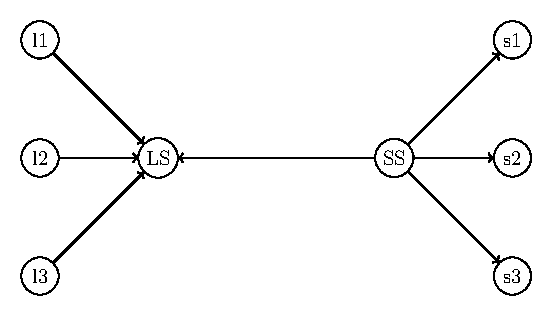
\includegraphics[scale=0.8]{Fig4.pdf}
	\end{center}
	
      We assume the weight of the central arc to be $0$ since it appears in every route,
      its value does not matter when considering affectations. Collisions between messages can 
      only appear at node $c_s$ on the way forward and at node $c_t$ on the way back. \\
      In such a topology, there is only two possible collision points between the routes : $c_s$ and $c_t$. To avoid collisions, we only have to check if there is no collisions in a period on those two points.
      Let us take a period P for each central nodes, that are called the {\bf forward period} and the {\bf backward period} for, respectively $c_s$ and $c_t$. A message issued by the source $s_1$ at time $m_{s_1}$ will reach $c_s$ at time $m_{s_1} + t(c_s,r_{s_1})$ in the forward period, and  $c_t$ at time $m_{{\cal C}(s_1)} + t(c_t,r_{{\cal C}(s_1)})$ in the backward period.
      A $(P,\tau)$-periodic affectation consist in choosing $\forall i \in n, m_i$, and $m_{{\cal C}(s_i)}$ such that, for any couples of routes $(r_{s_j}, r_{s_k}), j,k \in n$,
      we have $[t(c_s,r_j)] \cap [t(c_s,r_k)] = \emptyset$.
      and for any couples of routes $(r_{{\cal C}(s_j)}, r_{{\cal C}(s_k)}), j,k \in n$, we have $[t(c_s,r_{{\cal C}(s_j)})] \cap [t(c_s,r_{{\cal C}(s_k)})] = \emptyset$
%       
%   \todo{Définir la forward period et la backward period et dire à quoi correspond une affectation en terme de forward et backward period (placement de messages dans la première période}     
%       Therefore, 
%       finding an $(P,\tau)$-periodic affectation without collision, is equivalent to fix ...

      
%       
%       between the two central nodes is simplified in the forthcoming calculations.
%       Let us call {\bf SN} (source node) the central node connected to leaves, and {\bf SN} (sources node), the one connected to sources. The period in those nodes are respectively called {\em forward period}, and {\em backward period}.
      

  \subsection{Solving PALL without waiting times}
  
  In this subsection, we deal with a simpler version of the problem PALL.
  We ask for a $(P,\tau)$-periodic affectation with all waiting times equal to $0$. 
  In that case $T_{max}$ is not relevant anymore. Since $w_i=0$, choosing $m_i$, the offset of the route from
  $s_i$ to $t_i$, also sets the offset of the route from $t_i$ to $s_i$ to $m_i + \lambda(r_i)$.
  Moreover, in this context the weight of the arcs from $s_i$ to $c_s$ have no impact, therefore we assume they are 
  equal to $0$. \\
  For those reasons, in this case, we only have to consider the forward and backward periods. Indeed, setting the offset $m_{s_i}$ in the forward period automatically set the offsets $m_{{\cal C}(s_i)}$ in the backward period.
  The goal is now to put messages in the forward periods such that there is no collisions in the both periods.\\
  In this section, the offsets $m_{s_i}$ are in reality $[t(c_s,r_{s_i})]$, but to find the real values, there is just to change the values of the offset considering the delay of the arcs $(s_i, c_s) , \forall i$.
  
  
    \subsubsection{Shortest-longest policy}
    
    \paragraph{Algo}
    We present a simple policy, which works when the period is large with regards to the delay of the routes.
    Send the messages in order from the shortest route to the longest route, on after each others in the forward period, without any slots between two messages, that is $m_{s_i} = \tau.i$, if the routes $r_i$ are ordered by $\lambda(r_i)$ from the shortest to the longest one. 
      
      
The message using the shortest route is sent before the others, so it comes back to the central node before the following ones.
Then, the second message is sent before the others, and also will be back before the third etc... 
Because the second message is sent $\tau$ slots after the first message ($m_{s_2} = m_{s_1} + \tau$, it comes back after
the end of the message one: $m_{s_1}+ \tau + 2.\lambda(r_{s_1}) \le m_{s_2} + 2.\lambda(r_{s_2})$ because of $\lambda(r_{s_2}) \ge \lambda(r_{s_1})$.

      \paragraph{Period}
      To ensure that there is no collisions in the backward period, we must ensure that the last message will not collide with the first message of the next period. We have to find the minimum period P such that the last message have totally came back before P slots after the first message.
      
      The this policy ensure us a period of $$P = \tau * n + 2(\lambda(r_{s_{n-1}}) - \lambda(r_{s_0}))$$ if routes $\{r_0,...,r_{s_{n-1}}\}$ are ordered
from the shortest to the longest. 
 \begin{proof}
We have to calculate the time taken by the last message to reach $c_t$. $2.\lambda(r_{s_0})$ is the first slot in which the first message is coming back in the backward period,
and 2$\lambda(r_{s_{n-1}}) + n . \tau $ is the time at which the last message has totally passed the switch.
Therefore, the period only depends of the difference between the longest and the shortest route: the larger this value is, the larger
the period is.
  \end{proof}    
   
    \subsubsection{Greedy Algorithm}
    
    We introduce a greedy algorithm to build a $(P,\tau)$-periodic affectation, which provably works when
    the period is large enough with regards to the number of routes and size of messages. In other words, 
    we can always find a solution when the network is far from saturated. 
    
    \begin{proposition}
    There is an algorithm, which finds a $(P,\tau)$-periodic affectation in time $O(n^2)$ when $P \geq 3n\tau$.
    \end{proposition}
    \begin{proof}
     We consider the forward period and cut it into consecutive macro slots of time of size $\tau$. The algorithm works in the following way: select the first route for which the offset as not been chosen. Try every offset which put the message in a  
     free macro slot in the forward period. It also fixes the position of a message in the backward period, and we choose the first offset which does not create a collision in the backward period. 
     Assume we choose the offset of the route $r_{k+1}$, we have  at least $3n - k$ free macro-slots, since $P \geq 3n\tau$. Each of these $3n - k$ possible offset values translates into $3n - k$ positions of messages in the backward period. All these positions are separated by at least $\tau$ slots. There are already $k$ messages of size $\tau$ in the backward period. One such message can intersect at most $2k$ potential positions, therefore  amongst the possible $3n - k$ positions, there are  $3n - k -2k$ which are without collision. Since $k < n$, one of the choice is without collision, which proves that the algorithm terminates and find a
     $(P,\tau)$-periodic affectation. 
     \end{proof}
      
      \begin{center}
      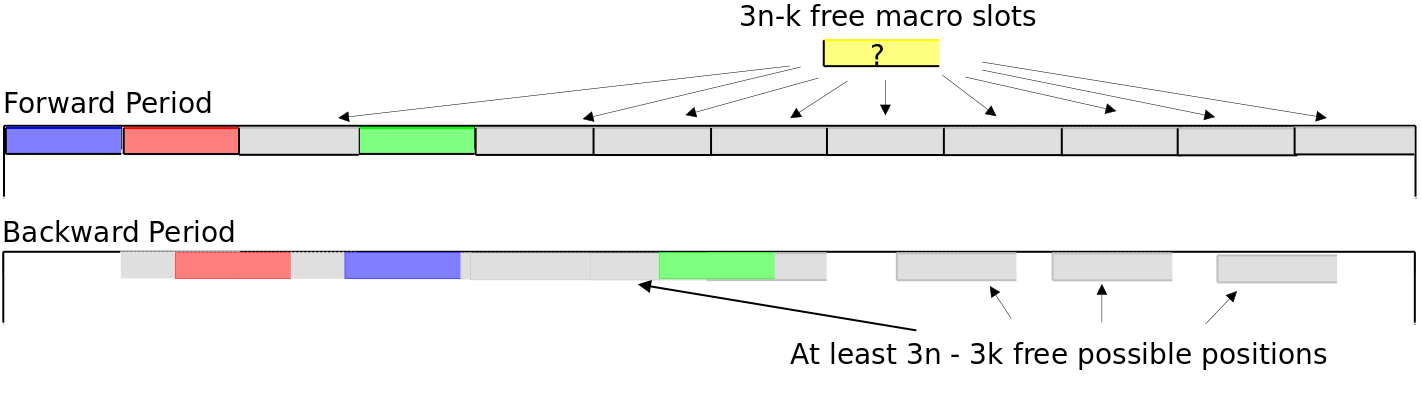
\includegraphics[scale=0.3]{ex3nt.png}
      \end{center}

    \todo{Avec une structure de données plus maligne on doit pouvoir faire n, non ?}
   
	\begin{algorithm}[H]
	\caption{Greedy affectation}
	\begin{algorithmic}
	\REQUIRE ${\cal R}_{\cal C}$, period $P$
	\ENSURE A P-periodic affectation in p $\leq P$, or FAILURE
	\STATE $P1[P]$ slots of size $\tau$ in forward period.
	\STATE $P2[P]$ slots  of size $\tau$ in backward period.
	\FORALL{source i in S }

	\FORALL{slot j in P1}

	\IF{$P1[j]$ is free AND $P2[j+\lambda(r_i)]$ is free}

	
	\STATE $m_{s_i} \leftarrow j$
	\ENDIF


	\IF{No intervals are found for i}
	\STATE return FAILURE
	\ENDIF
	\ENDFOR

	\ENDFOR

	\end{algorithmic}
	\end{algorithm}
%       \paragraph{Period}
% 	This algorithm gives us a solution without waiting times in a maximum period $3.\tau.c$, if we have $c$ routes.\\
% 	Suppose that we have a period of $3.\tau.c$ slots, divided in $\tau$ macro-slots. Put a message in the first slot of size $\tau$ in the forward period, such that the corresponding area in the backward period is free.This message takes at most 2 slots of time $\tau$ in the backward period.\\

% 	When $k < c$ messages are put in the forward period, and we want to add another message, there is $3.c - k$ free slots of size $\tau$ in the forward period. Those $3.c - k$ gives us $3.c - k$ possible slots in the backward periods.\\
% 	The $k$ messages uses at most $2k$ slots of size $\tau$ used in the backward period. Since $k<c$,  $2k < 3.c - k$, thus using the pigeonhole principle, there is at least one free slot in the backward period for the new message.
	
    \subsubsection{Exhaustive generation}
	\begin{algorithm}[H]
	\caption{Exhaustive Generation}  
	\begin{algorithmic}
	\REQUIRE A routage graph ${\cal R}_{\cal C}$, period $P$, packet size $\tau$
	\ENSURE $(P,\tau)$-periodic affectation of ${\cal R}_{\cal C}$
	\STATE Forward-budget $\leftarrow$ $P$ - n * $\tau$
	\STATE Backward-budget $\leftarrow$ $P$ - n * $\tau$
	\STATE Free-Intervals $\leftarrow$ list of free intervals, init to $[0;P[$
	\FORALL{route i in  ${\cal R}_{\cal C}$}
	\FORALL{j in Free-Intervals }
	\IF{Message of the route i does not collides with scheduled routes}
	\STATE $m_{s_i} \leftarrow $ the first slot of Free-Intervals[j]
	\STATE Split the Free-Intervals considering the new packet
	\STATE Forward-budget $\leftarrow$ Forward-budget - {\em lost size}
	\STATE Backward-budget $\leftarrow$ Backward-budget - {\em lost size}
	\STATE call Exhaustive Generation on remaining routes
	\ENDIF
	\ENDFOR
	\ENDFOR


      \end{algorithmic}
      \end{algorithm}
      {\bf {\em Lost size}}, is the size lost when an interval is too few to put another packet. Ex : if the interval [250;3250[ receives a packet of size 2500, there is 500 slots lost, because there is no way to uses the slots for another packet.\\
      
	    
      This algorithm enumerates all the solutions by traversing a tree. The leaves of the tree are 
      the $(P\tau)$-periodic affectations, and the nodes are partial solutions. A partial solution is a choice of a starting time for a subset of the routes.
      For each route, the algorithm tries every possible starting offset until it finds one available (that allows the message to come back without collisions). When a route have been scheduled, it take another route that have not been scheduled yet.
      This creates a new sub-tree in which the algorithm will try every possible starting offset too, and create a sub-tree on the following route too.
      If no offset are available for a route, this means that the partial solution is not good, so the algorithm backtracks over the tree that is,
      it goes back to the father of the current sub-tree.
      Once a leaf is obtained, the algorithm stops and return the scheduling.\\      
      To reduce the number of useless calculation, in each time we add another packet, we consider the lost size in both periods, thus, we know when a period has no many great enough free area to put a packet.

    \subsubsection{Results}
      Resultats des simulations : Shortest-longest optimal pour ces parametres.
      
   \subsection{Allowing waiting times}
     \subsubsection{Intro}
	Importance des waiting times quand la période est donnée (Résultats D'éxepriences et preuve avec l'exemple)
     \subsubsection{LSG}
     

To find a solution allowing waiting times, the following heuristic is suggested:

On leaves switch, the messages are scheduled so that they are following each others, from the one using the longest route, to the one using the shortest route.

On sources switch, the politic is the following one, after setting the clock to 0, do:
\begin{enumerate}
 \item To be eligible, a job needs to be able to come back on the switch at the current clock (if clock = 0, take the first message able to come back).
 \item Between the eligible jobs, schedule first the one which has the longest route gives it the starting time $o_i = clock$.
 \item Update the clock at the time in which the scheduled task is over: $$clock = clock + message\ length$$.
\end{enumerate}

This algorithm defines the offsets of the first $P$-periodic affectation by sending the messages from the longest route to the shortest route, then it uses a greedy algorithm to schedule the messages in the second $P$-periodic affectation. We denote this algorithm by LSG (Longest Shortest + Greedy).

\begin{algorithm}[H]
\caption{LSG}
\begin{algorithmic}
\REQUIRE Matched graph $N$, period $P$, packet size T
\ENSURE 2way Trip affectation in P
\STATE clock $\leftarrow$ 0
\FORALL{route i in $\rho$ from the longest to the shortest }
\STATE  $m_i \leftarrow$ clock
\STATE clock $\leftarrow$ clock + T
\ENDFOR
\STATE clock $\leftarrow$ 0
\STATE take i such that $r_i$ is the first route to come back in sources switch
\STATE $o_i \leftarrow $ clock;
\STATE clock $\leftarrow$ $a_i$ + T
\WHILE{there is a route which has no $w_i$}
\STATE take i such that $r_i$ is the eligible route.
\STATE $o_i \leftarrow $ clock - $a_i$;
\STATE clock $\leftarrow$ clock + T

\ENDWHILE

\end{algorithmic}
\end{algorithm}

	\paragraph{Algorithm}
	\paragraph{Analysis}
	  Parler de LSO et expliquer pourquoi LSG mieux avec nos params
     \subsubsection{Results}
	 \paragraph{Random}
	 \paragraph{Distributions}
   
\section{Conclusion}


Open questions. Can we improve the results if:
\begin{itemize}
 \item The routes are smaller than the size of a message. 
\item The routes are smaller than the period.
\item The largest difference between two routes is smallest than one of these parameters
\end{itemize}

 On a general graph:
 
\begin{itemize}
\item The routing is coherent
 \item The graph is symmetric
\end{itemize}


\bibliographystyle{plain}
\bibliography{Sources.bib}


\end{document}
